\documentclass[twoside]{book}

% Packages required by doxygen
\usepackage{fixltx2e}
\usepackage{calc}
\usepackage{doxygen}
\usepackage[export]{adjustbox} % also loads graphicx
\usepackage{graphicx}
\usepackage[utf8]{inputenc}
\usepackage{makeidx}
\usepackage{multicol}
\usepackage{multirow}
\PassOptionsToPackage{warn}{textcomp}
\usepackage{textcomp}
\usepackage[nointegrals]{wasysym}
\usepackage[table]{xcolor}

% Font selection
\usepackage[T1]{fontenc}
\usepackage[scaled=.90]{helvet}
\usepackage{courier}
\usepackage{amssymb}
\usepackage{sectsty}
\renewcommand{\familydefault}{\sfdefault}
\allsectionsfont{%
  \fontseries{bc}\selectfont%
  \color{darkgray}%
}
\renewcommand{\DoxyLabelFont}{%
  \fontseries{bc}\selectfont%
  \color{darkgray}%
}
\newcommand{\+}{\discretionary{\mbox{\scriptsize$\hookleftarrow$}}{}{}}

% Page & text layout
\usepackage{geometry}
\geometry{%
  a4paper,%
  top=2.5cm,%
  bottom=2.5cm,%
  left=2.5cm,%
  right=2.5cm%
}
\tolerance=750
\hfuzz=15pt
\hbadness=750
\setlength{\emergencystretch}{15pt}
\setlength{\parindent}{0cm}
\setlength{\parskip}{0.2cm}
\makeatletter
\renewcommand{\paragraph}{%
  \@startsection{paragraph}{4}{0ex}{-1.0ex}{1.0ex}{%
    \normalfont\normalsize\bfseries\SS@parafont%
  }%
}
\renewcommand{\subparagraph}{%
  \@startsection{subparagraph}{5}{0ex}{-1.0ex}{1.0ex}{%
    \normalfont\normalsize\bfseries\SS@subparafont%
  }%
}
\makeatother

% Headers & footers
\usepackage{fancyhdr}
\pagestyle{fancyplain}
\fancyhead[LE]{\fancyplain{}{\bfseries\thepage}}
\fancyhead[CE]{\fancyplain{}{}}
\fancyhead[RE]{\fancyplain{}{\bfseries\leftmark}}
\fancyhead[LO]{\fancyplain{}{\bfseries\rightmark}}
\fancyhead[CO]{\fancyplain{}{}}
\fancyhead[RO]{\fancyplain{}{\bfseries\thepage}}
\fancyfoot[LE]{\fancyplain{}{}}
\fancyfoot[CE]{\fancyplain{}{}}
\fancyfoot[RE]{\fancyplain{}{\bfseries\scriptsize Generated on Fri Dec 11 2015 21\+:01\+:51 for My Project by Doxygen }}
\fancyfoot[LO]{\fancyplain{}{\bfseries\scriptsize Generated on Fri Dec 11 2015 21\+:01\+:51 for My Project by Doxygen }}
\fancyfoot[CO]{\fancyplain{}{}}
\fancyfoot[RO]{\fancyplain{}{}}
\renewcommand{\footrulewidth}{0.4pt}
\renewcommand{\chaptermark}[1]{%
  \markboth{#1}{}%
}
\renewcommand{\sectionmark}[1]{%
  \markright{\thesection\ #1}%
}

% Indices & bibliography
\usepackage{natbib}
\usepackage[titles]{tocloft}
\setcounter{tocdepth}{3}
\setcounter{secnumdepth}{5}
\makeindex

% Hyperlinks (required, but should be loaded last)
\usepackage{ifpdf}
\ifpdf
  \usepackage[pdftex,pagebackref=true]{hyperref}
\else
  \usepackage[ps2pdf,pagebackref=true]{hyperref}
\fi
\hypersetup{%
  colorlinks=true,%
  linkcolor=blue,%
  citecolor=blue,%
  unicode%
}

% Custom commands
\newcommand{\clearemptydoublepage}{%
  \newpage{\pagestyle{empty}\cleardoublepage}%
}


%===== C O N T E N T S =====

\begin{document}

% Titlepage & ToC
\hypersetup{pageanchor=false,
             bookmarks=true,
             bookmarksnumbered=true,
             pdfencoding=unicode
            }
\pagenumbering{roman}
\begin{titlepage}
\vspace*{7cm}
\begin{center}%
{\Large My Project }\\
\vspace*{1cm}
{\large Generated by Doxygen 1.8.10}\\
\vspace*{0.5cm}
{\small Fri Dec 11 2015 21:01:51}\\
\end{center}
\end{titlepage}
\clearemptydoublepage
\tableofcontents
\clearemptydoublepage
\pagenumbering{arabic}
\hypersetup{pageanchor=true}

%--- Begin generated contents ---
\chapter{Hierarchical Index}
\section{Class Hierarchy}
This inheritance list is sorted roughly, but not completely, alphabetically\+:\begin{DoxyCompactList}
\item \contentsline{section}{Greeting}{\pageref{struct_greeting}}{}
\item \contentsline{section}{Player}{\pageref{class_player}}{}
\item \contentsline{section}{Player\+Data}{\pageref{struct_player_data}}{}
\item \contentsline{section}{Simple\+Vector$<$ T $>$}{\pageref{class_simple_vector}}{}
\item \contentsline{section}{Unit}{\pageref{class_unit}}{}
\begin{DoxyCompactList}
\item \contentsline{section}{Enemy\+Unit}{\pageref{class_enemy_unit}}{}
\begin{DoxyCompactList}
\item \contentsline{section}{Boss\+Unit}{\pageref{class_boss_unit}}{}
\item \contentsline{section}{Crap\+Unit}{\pageref{class_crap_unit}}{}
\begin{DoxyCompactList}
\item \contentsline{section}{Crap\+Unit\+Elite}{\pageref{class_crap_unit_elite}}{}
\end{DoxyCompactList}
\item \contentsline{section}{Moderate\+Unit}{\pageref{class_moderate_unit}}{}
\begin{DoxyCompactList}
\item \contentsline{section}{Moderate\+Unit\+Elite}{\pageref{class_moderate_unit_elite}}{}
\end{DoxyCompactList}
\end{DoxyCompactList}
\end{DoxyCompactList}
\item \contentsline{section}{Weapon}{\pageref{class_weapon}}{}
\end{DoxyCompactList}

\chapter{Class Index}
\section{Class List}
Here are the classes, structs, unions and interfaces with brief descriptions\+:\begin{DoxyCompactList}
\item\contentsline{section}{\hyperlink{struct_records}{Records} }{\pageref{struct_records}}{}
\end{DoxyCompactList}

\chapter{Class Documentation}
\hypertarget{class_boss_unit}{}\section{Boss\+Unit Class Reference}
\label{class_boss_unit}\index{Boss\+Unit@{Boss\+Unit}}
Inheritance diagram for Boss\+Unit\+:\begin{figure}[H]
\begin{center}
\leavevmode
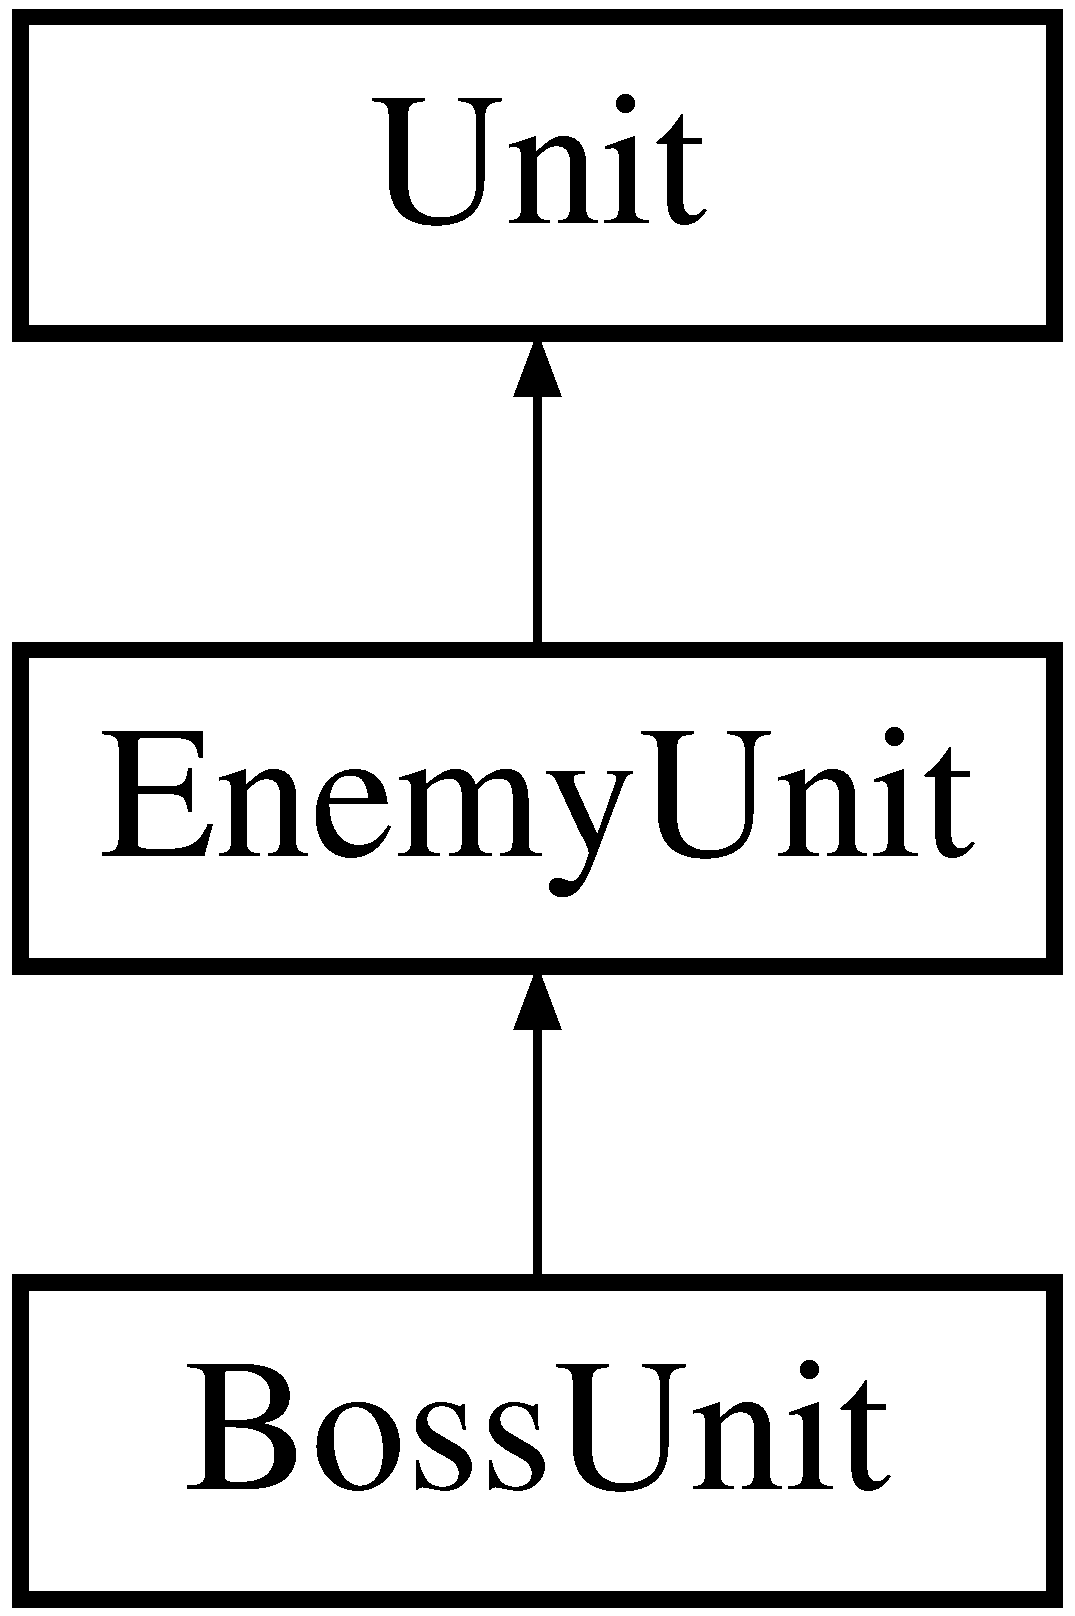
\includegraphics[height=3.000000cm]{class_boss_unit}
\end{center}
\end{figure}
\subsection*{Public Member Functions}
\begin{DoxyCompactItemize}
\item 
\hypertarget{class_boss_unit_a2d4dc82113ddce7c27cd3ea6eeb6cc17}{}void {\bfseries set\+Bon} (string)\label{class_boss_unit_a2d4dc82113ddce7c27cd3ea6eeb6cc17}

\item 
\hypertarget{class_boss_unit_add584e941cb3823fdc0d82c706bf9ed5}{}void {\bfseries set\+Spec} (string)\label{class_boss_unit_add584e941cb3823fdc0d82c706bf9ed5}

\item 
\hypertarget{class_boss_unit_a0eecd42028e0d4ff0334c2807875c8e9}{}string {\bfseries get\+Bon} ()\label{class_boss_unit_a0eecd42028e0d4ff0334c2807875c8e9}

\item 
\hypertarget{class_boss_unit_af3cdfcec977cb32bb5704b0388daeca9}{}string {\bfseries get\+Spec} ()\label{class_boss_unit_af3cdfcec977cb32bb5704b0388daeca9}

\end{DoxyCompactItemize}
\subsection*{Additional Inherited Members}


The documentation for this class was generated from the following files\+:\begin{DoxyCompactItemize}
\item 
Boss\+Unit.\+h\item 
Boss\+Unit.\+cpp\end{DoxyCompactItemize}

\hypertarget{class_crap_unit}{}\section{Crap\+Unit Class Reference}
\label{class_crap_unit}\index{Crap\+Unit@{Crap\+Unit}}
Inheritance diagram for Crap\+Unit\+:\begin{figure}[H]
\begin{center}
\leavevmode
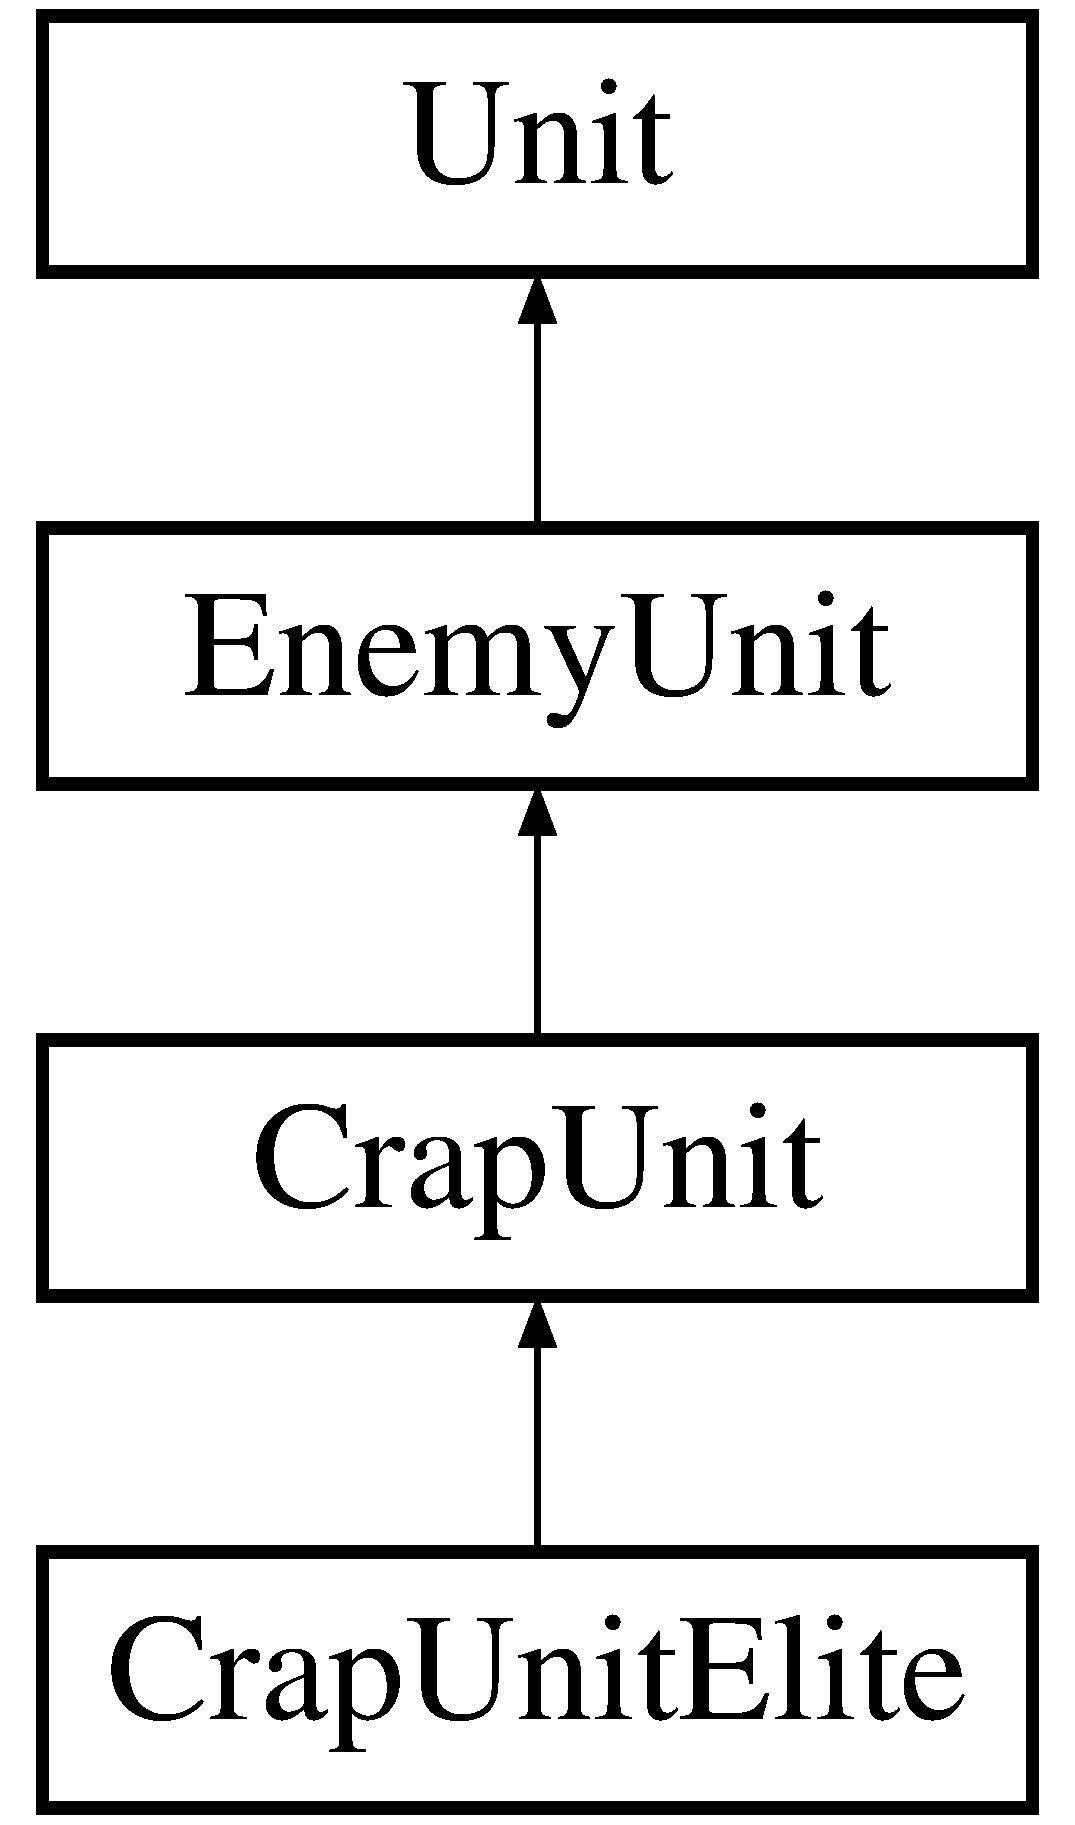
\includegraphics[height=4.000000cm]{class_crap_unit}
\end{center}
\end{figure}
\subsection*{Public Member Functions}
\begin{DoxyCompactItemize}
\item 
\hypertarget{class_crap_unit_a2f1a878e3b26dd87a7a205289a4b2c24}{}{\bfseries Crap\+Unit} (string, int, int, string, string)\label{class_crap_unit_a2f1a878e3b26dd87a7a205289a4b2c24}

\item 
\hypertarget{class_crap_unit_a417bd87e2d41efef62c125fa3c8e2c1a}{}void {\bfseries set\+Type} (string)\label{class_crap_unit_a417bd87e2d41efef62c125fa3c8e2c1a}

\item 
\hypertarget{class_crap_unit_aa4a586bf92c873126bc80376beef952c}{}void {\bfseries set\+Weak} (string)\label{class_crap_unit_aa4a586bf92c873126bc80376beef952c}

\item 
\hypertarget{class_crap_unit_a7bd065772872b94fb404b8a546420fab}{}string {\bfseries get\+Type} ()\label{class_crap_unit_a7bd065772872b94fb404b8a546420fab}

\item 
\hypertarget{class_crap_unit_a93ead139bd06781739523304e5a63e21}{}string {\bfseries get\+Weak} ()\label{class_crap_unit_a93ead139bd06781739523304e5a63e21}

\end{DoxyCompactItemize}
\subsection*{Protected Attributes}
\begin{DoxyCompactItemize}
\item 
\hypertarget{class_crap_unit_a6b75381e9d70b4b5ac33d8c1d66b925d}{}string {\bfseries type}\label{class_crap_unit_a6b75381e9d70b4b5ac33d8c1d66b925d}

\item 
\hypertarget{class_crap_unit_ab98d883fdebd069691caebc847b0a65d}{}string {\bfseries weakness}\label{class_crap_unit_ab98d883fdebd069691caebc847b0a65d}

\end{DoxyCompactItemize}
\subsection*{Additional Inherited Members}


The documentation for this class was generated from the following files\+:\begin{DoxyCompactItemize}
\item 
Crap\+Unit.\+h\item 
Crap\+Unit.\+cpp\end{DoxyCompactItemize}

\hypertarget{class_crap_unit_elite}{}\section{Crap\+Unit\+Elite Class Reference}
\label{class_crap_unit_elite}\index{Crap\+Unit\+Elite@{Crap\+Unit\+Elite}}
Inheritance diagram for Crap\+Unit\+Elite\+:\begin{figure}[H]
\begin{center}
\leavevmode
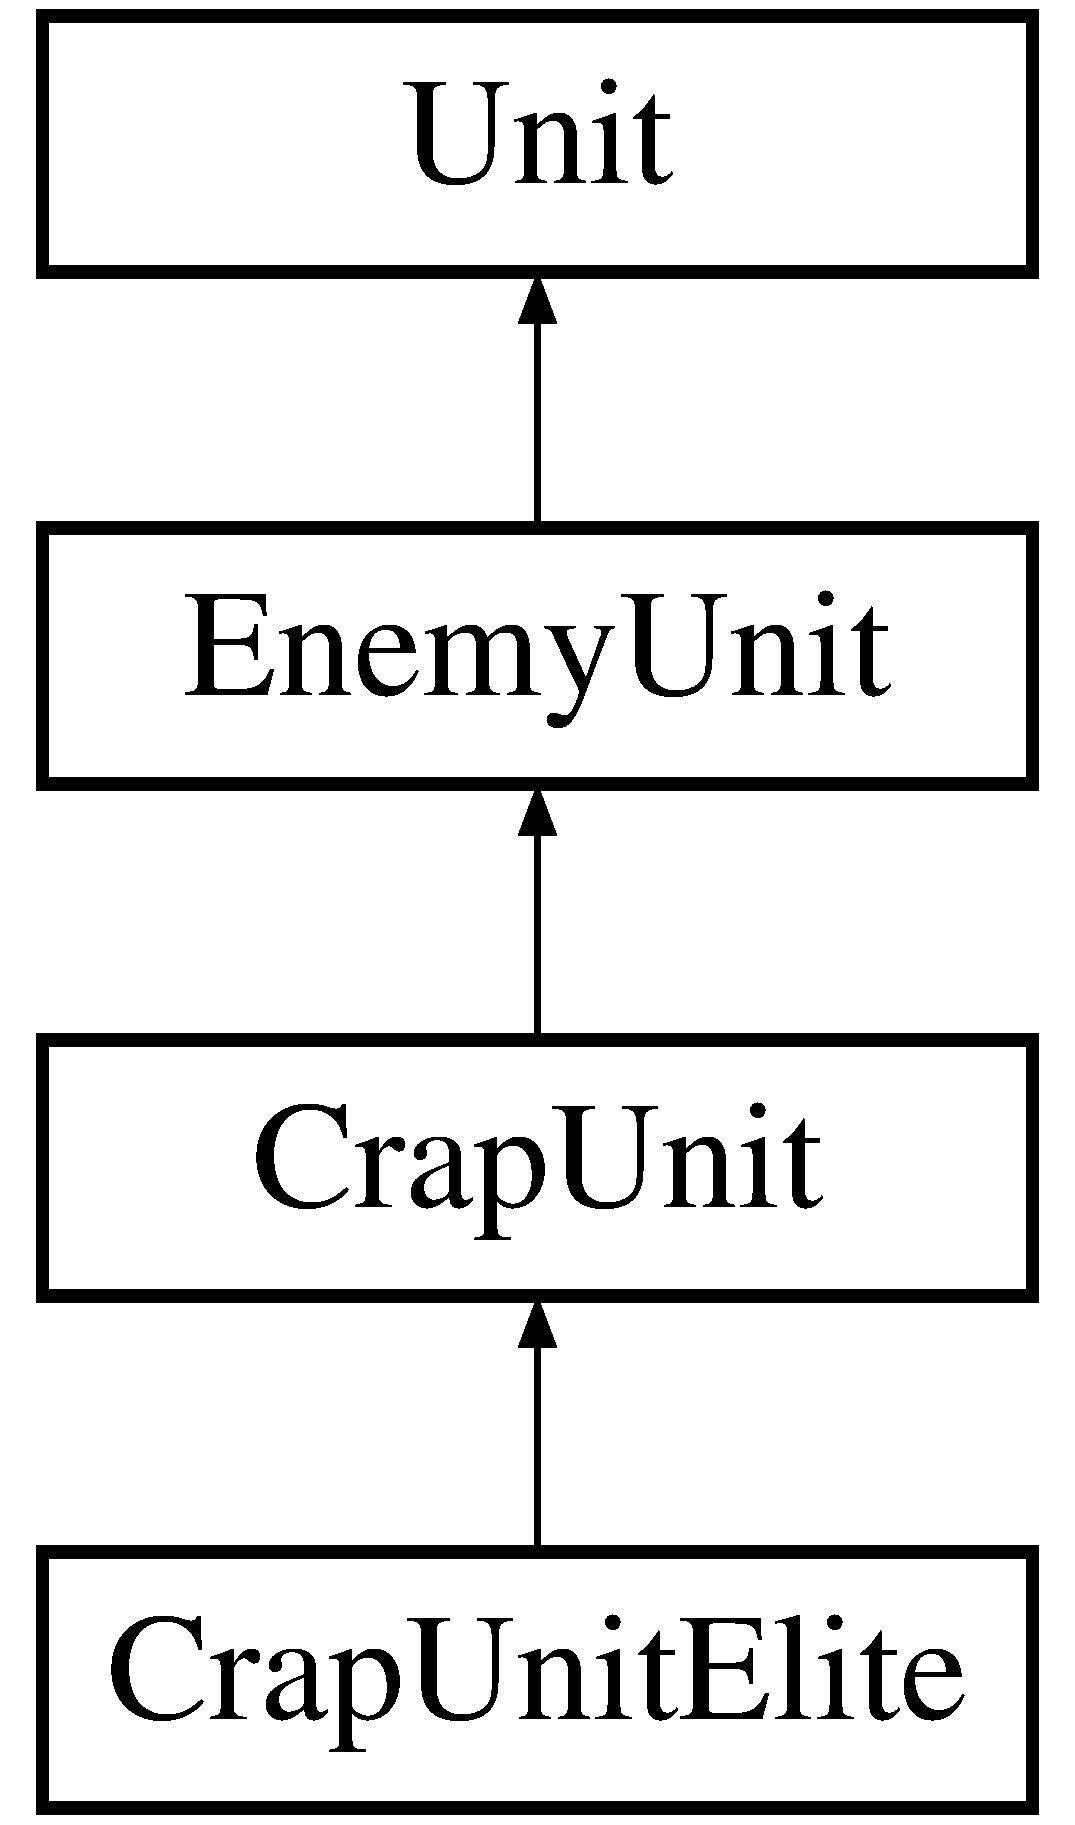
\includegraphics[height=4.000000cm]{class_crap_unit_elite}
\end{center}
\end{figure}
\subsection*{Public Member Functions}
\begin{DoxyCompactItemize}
\item 
\hypertarget{class_crap_unit_elite_af7be3a6657521fcc0f069885bed1c22e}{}{\bfseries Crap\+Unit\+Elite} (string, int, int, string, string, string)\label{class_crap_unit_elite_af7be3a6657521fcc0f069885bed1c22e}

\item 
\hypertarget{class_crap_unit_elite_a6b51bc5cdaadce0625be6cd97ac0b100}{}void {\bfseries set\+Bon} (string)\label{class_crap_unit_elite_a6b51bc5cdaadce0625be6cd97ac0b100}

\item 
\hypertarget{class_crap_unit_elite_a9ed4d3390c965cc54a46678465de15da}{}string {\bfseries get\+Bon} ()\label{class_crap_unit_elite_a9ed4d3390c965cc54a46678465de15da}

\end{DoxyCompactItemize}
\subsection*{Additional Inherited Members}


The documentation for this class was generated from the following files\+:\begin{DoxyCompactItemize}
\item 
Crap\+Unit\+Elite.\+h\item 
Crap\+Unit\+Elite.\+cpp\end{DoxyCompactItemize}

\hypertarget{class_enemy_unit}{}\section{Enemy\+Unit Class Reference}
\label{class_enemy_unit}\index{Enemy\+Unit@{Enemy\+Unit}}
Inheritance diagram for Enemy\+Unit\+:\begin{figure}[H]
\begin{center}
\leavevmode
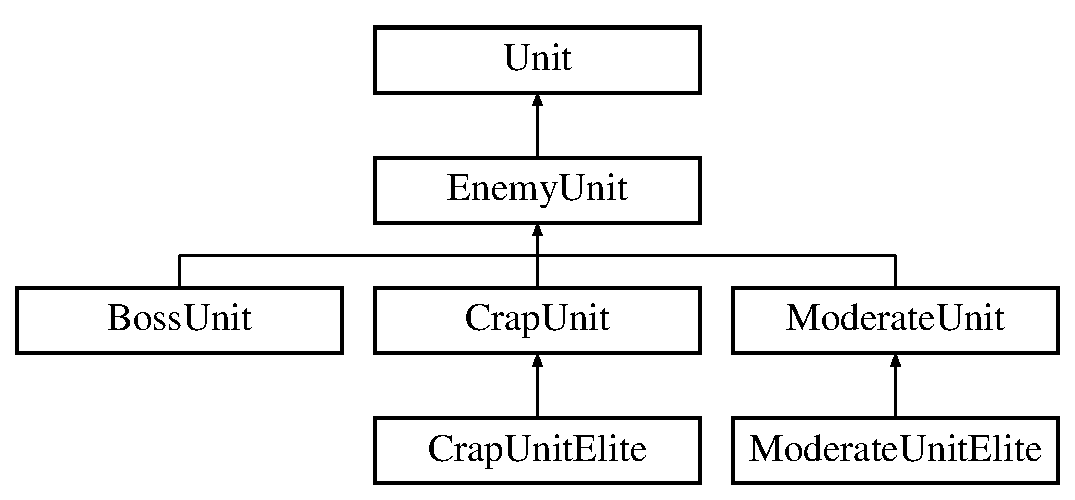
\includegraphics[height=4.000000cm]{class_enemy_unit}
\end{center}
\end{figure}
\subsection*{Public Member Functions}
\begin{DoxyCompactItemize}
\item 
\hypertarget{class_enemy_unit_a3ae128f102ada75eb2a6e852473142a9}{}{\bfseries Enemy\+Unit} (string, int, int)\label{class_enemy_unit_a3ae128f102ada75eb2a6e852473142a9}

\item 
\hypertarget{class_enemy_unit_afb5ef9ae0126b962b832f11a0dc580fe}{}void {\bfseries set\+Name} (string)\label{class_enemy_unit_afb5ef9ae0126b962b832f11a0dc580fe}

\item 
\hypertarget{class_enemy_unit_ac00dac68029c40282e0a1d68e84da6c5}{}string {\bfseries get\+Name} ()\label{class_enemy_unit_ac00dac68029c40282e0a1d68e84da6c5}

\item 
\hypertarget{class_enemy_unit_af541efec09d48c3188abb76a9dc3c6db}{}void {\bfseries set\+Hlth} (int)\label{class_enemy_unit_af541efec09d48c3188abb76a9dc3c6db}

\item 
\hypertarget{class_enemy_unit_a6b36534e52356d7ef96c17f1b0fc7dc9}{}int {\bfseries get\+Hlth} ()\label{class_enemy_unit_a6b36534e52356d7ef96c17f1b0fc7dc9}

\item 
\hypertarget{class_enemy_unit_a69f40fbd4d6cfff6d85d67efd4bedaea}{}void {\bfseries set\+Dps} (int)\label{class_enemy_unit_a69f40fbd4d6cfff6d85d67efd4bedaea}

\item 
\hypertarget{class_enemy_unit_a0410203a93c5daaf536a4a71e853eb5a}{}int {\bfseries get\+Dps} ()\label{class_enemy_unit_a0410203a93c5daaf536a4a71e853eb5a}

\item 
\hypertarget{class_enemy_unit_adf121b3d60198679616611b8a354003b}{}void {\bfseries take\+Dmg} (int)\label{class_enemy_unit_adf121b3d60198679616611b8a354003b}

\item 
\hypertarget{class_enemy_unit_a46f445bef004fbee07ec13529c4dea62}{}int {\bfseries get\+Hate} ()\label{class_enemy_unit_a46f445bef004fbee07ec13529c4dea62}

\end{DoxyCompactItemize}
\subsection*{Protected Attributes}
\begin{DoxyCompactItemize}
\item 
\hypertarget{class_enemy_unit_a30dd4f42740fb170e78bda8720740eda}{}string {\bfseries name}\label{class_enemy_unit_a30dd4f42740fb170e78bda8720740eda}

\item 
\hypertarget{class_enemy_unit_a94adccb46717e178ef57b0c88b5198c1}{}int {\bfseries health}\label{class_enemy_unit_a94adccb46717e178ef57b0c88b5198c1}

\item 
\hypertarget{class_enemy_unit_ac31f29870ecf7f5feaf23aa650d0c6a4}{}int {\bfseries dps}\label{class_enemy_unit_ac31f29870ecf7f5feaf23aa650d0c6a4}

\end{DoxyCompactItemize}
\subsection*{Static Protected Attributes}
\begin{DoxyCompactItemize}
\item 
\hypertarget{class_enemy_unit_a69dc9271045ac595cf03f9d5584a3961}{}static string {\bfseries allegiance} =\char`\"{}The Dark Lord Cthulhu\char`\"{}\label{class_enemy_unit_a69dc9271045ac595cf03f9d5584a3961}

\end{DoxyCompactItemize}


The documentation for this class was generated from the following files\+:\begin{DoxyCompactItemize}
\item 
Enemy\+Unit.\+h\item 
Enemy\+Unit.\+cpp\end{DoxyCompactItemize}

\hypertarget{struct_greeting}{}\section{Greeting Struct Reference}
\label{struct_greeting}\index{Greeting@{Greeting}}


The documentation for this struct was generated from the following file\+:\begin{DoxyCompactItemize}
\item 
Greetings.\+h\end{DoxyCompactItemize}

\hypertarget{class_moderate_unit}{}\section{Moderate\+Unit Class Reference}
\label{class_moderate_unit}\index{Moderate\+Unit@{Moderate\+Unit}}
Inheritance diagram for Moderate\+Unit\+:\begin{figure}[H]
\begin{center}
\leavevmode
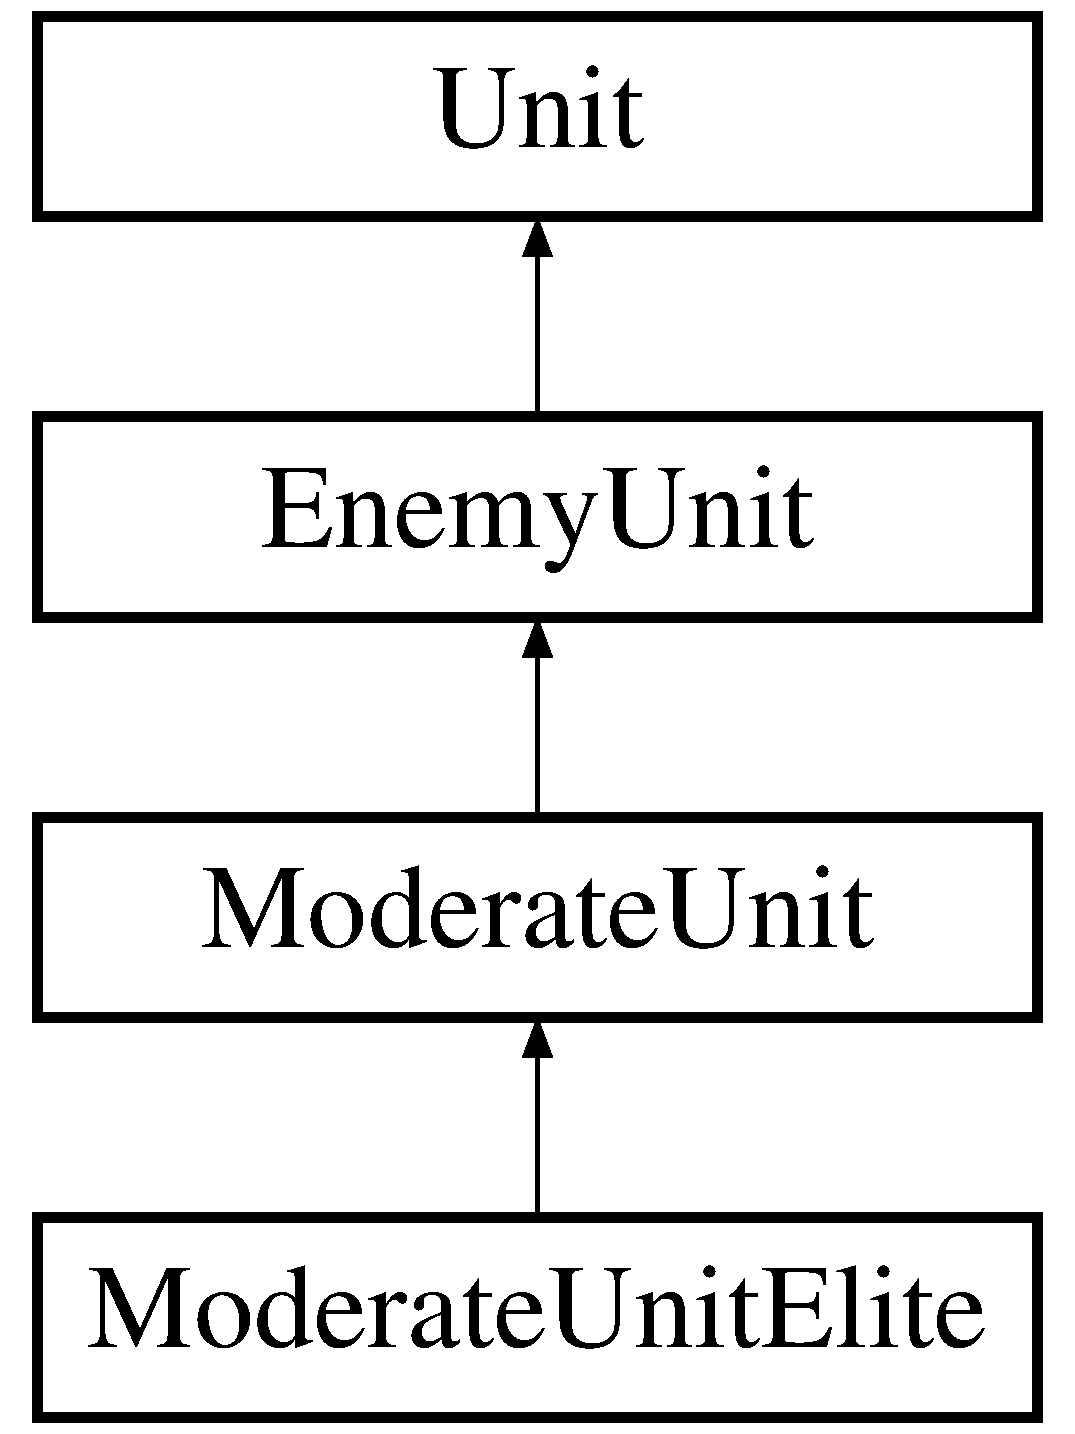
\includegraphics[height=4.000000cm]{class_moderate_unit}
\end{center}
\end{figure}
\subsection*{Public Member Functions}
\begin{DoxyCompactItemize}
\item 
\hypertarget{class_moderate_unit_af450a9f4bb904b9c5c3e22b05fd436f9}{}{\bfseries Moderate\+Unit} (string, int, int, string, string)\label{class_moderate_unit_af450a9f4bb904b9c5c3e22b05fd436f9}

\item 
\hypertarget{class_moderate_unit_a11a78a8ca570fdd48fafcbf98ec73a74}{}void {\bfseries set\+Type} (string)\label{class_moderate_unit_a11a78a8ca570fdd48fafcbf98ec73a74}

\item 
\hypertarget{class_moderate_unit_affd75b90bdf05302caf081f6abfc9f18}{}void {\bfseries set\+Weak} (string)\label{class_moderate_unit_affd75b90bdf05302caf081f6abfc9f18}

\item 
\hypertarget{class_moderate_unit_a20d91613d3f14a9c33a02adf6e844338}{}string {\bfseries get\+Type} ()\label{class_moderate_unit_a20d91613d3f14a9c33a02adf6e844338}

\item 
\hypertarget{class_moderate_unit_a0bb728728033b2809bd9ce7dbf4f2c48}{}string {\bfseries get\+Weak} ()\label{class_moderate_unit_a0bb728728033b2809bd9ce7dbf4f2c48}

\end{DoxyCompactItemize}
\subsection*{Protected Attributes}
\begin{DoxyCompactItemize}
\item 
\hypertarget{class_moderate_unit_ab703fcea9a80c008dd7c9db4cef239cd}{}string {\bfseries type}\label{class_moderate_unit_ab703fcea9a80c008dd7c9db4cef239cd}

\item 
\hypertarget{class_moderate_unit_a6986d68b88dda21f3f98074fa0727ee3}{}string {\bfseries weakness}\label{class_moderate_unit_a6986d68b88dda21f3f98074fa0727ee3}

\end{DoxyCompactItemize}
\subsection*{Additional Inherited Members}


The documentation for this class was generated from the following files\+:\begin{DoxyCompactItemize}
\item 
Moderate\+Unit.\+h\item 
Moderate\+Unit.\+cpp\end{DoxyCompactItemize}

\hypertarget{class_moderate_unit_elite}{}\section{Moderate\+Unit\+Elite Class Reference}
\label{class_moderate_unit_elite}\index{Moderate\+Unit\+Elite@{Moderate\+Unit\+Elite}}
Inheritance diagram for Moderate\+Unit\+Elite\+:\begin{figure}[H]
\begin{center}
\leavevmode
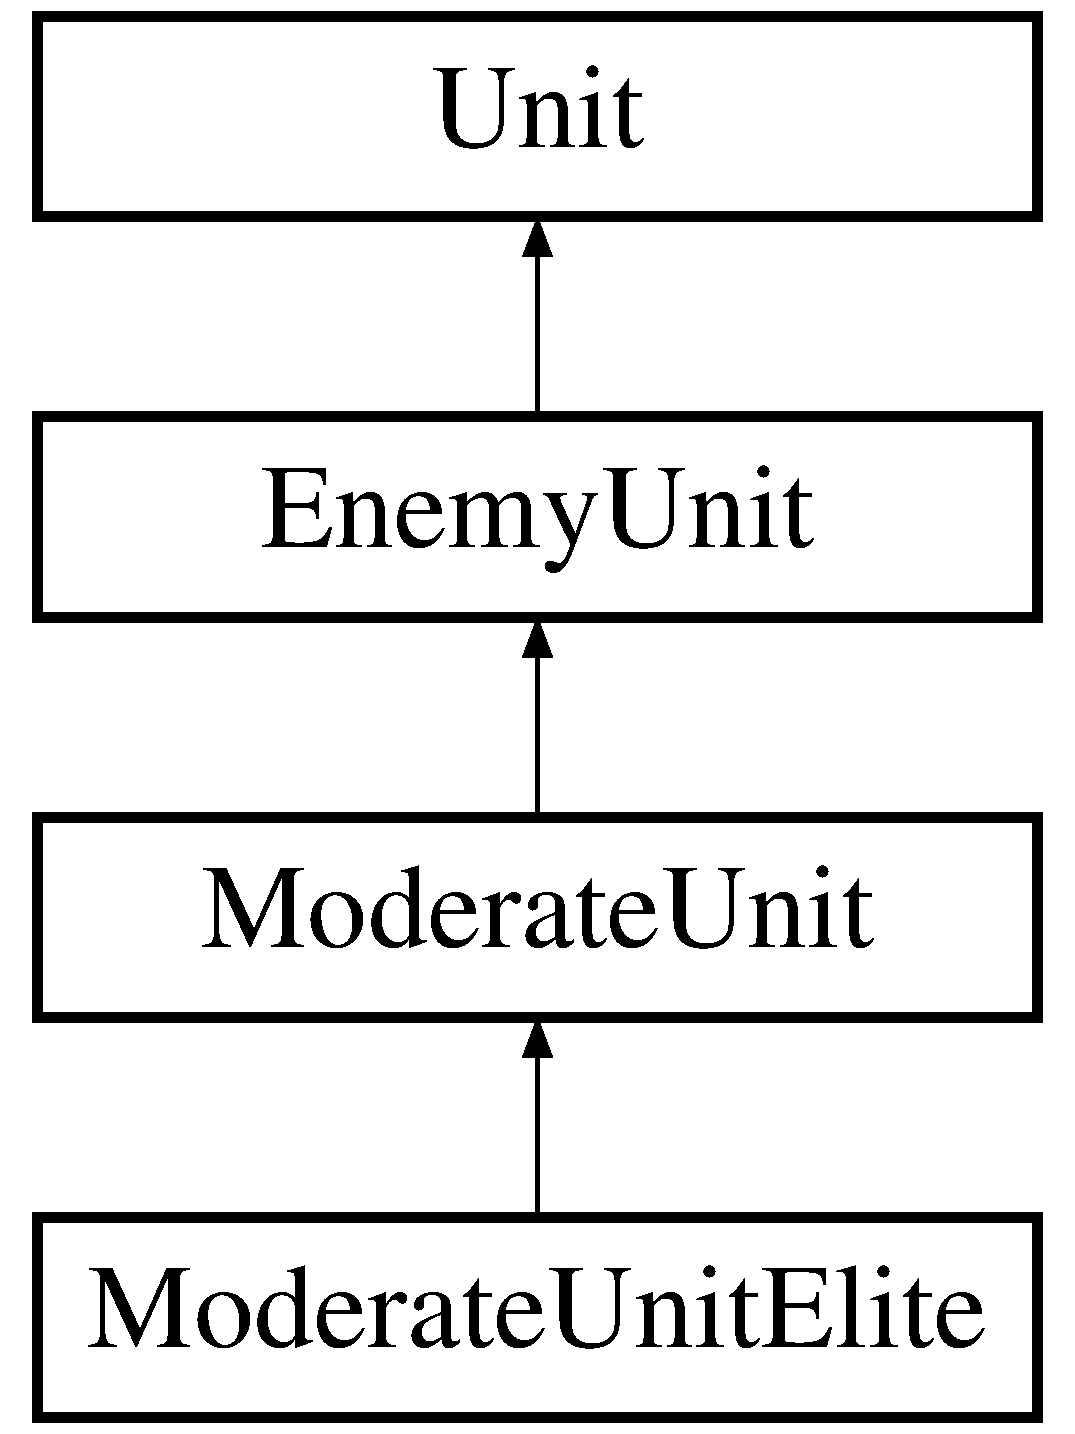
\includegraphics[height=4.000000cm]{class_moderate_unit_elite}
\end{center}
\end{figure}
\subsection*{Public Member Functions}
\begin{DoxyCompactItemize}
\item 
\hypertarget{class_moderate_unit_elite_a03d56dacbd2de505bd599b4dac1c5bcb}{}{\bfseries Moderate\+Unit\+Elite} (string, int, int, string, string)\label{class_moderate_unit_elite_a03d56dacbd2de505bd599b4dac1c5bcb}

\item 
\hypertarget{class_moderate_unit_elite_a1e9c5f1e34b5f1da8eb405c091a35188}{}void {\bfseries set\+Bon} (string)\label{class_moderate_unit_elite_a1e9c5f1e34b5f1da8eb405c091a35188}

\item 
\hypertarget{class_moderate_unit_elite_ac07b4185480f96ef5cf5f47f1eba35ce}{}string {\bfseries get\+Bon} ()\label{class_moderate_unit_elite_ac07b4185480f96ef5cf5f47f1eba35ce}

\end{DoxyCompactItemize}
\subsection*{Additional Inherited Members}


The documentation for this class was generated from the following files\+:\begin{DoxyCompactItemize}
\item 
Moderate\+Unit\+Elite.\+h\item 
Moderate\+Unit\+Elite.\+cpp\end{DoxyCompactItemize}

\hypertarget{class_player}{}\section{Player Class Reference}
\label{class_player}\index{Player@{Player}}
\subsection*{Public Member Functions}
\begin{DoxyCompactItemize}
\item 
\hypertarget{class_player_aaf1dcc6f6b07ba59fbbeb89f926cd0da}{}{\bfseries Player} (string, int)\label{class_player_aaf1dcc6f6b07ba59fbbeb89f926cd0da}

\item 
\hypertarget{class_player_a1f3ce001ef9ef11f684c1eda423afb30}{}{\bfseries Player} (string, int, int, string)\label{class_player_a1f3ce001ef9ef11f684c1eda423afb30}

\item 
\hypertarget{class_player_a8eaf43a2f2236b21d0101270ecca1483}{}void {\bfseries set\+Name} (string)\label{class_player_a8eaf43a2f2236b21d0101270ecca1483}

\item 
\hypertarget{class_player_a5a5c3fb613cdd39e0e5204b533b551e1}{}void {\bfseries set\+Hel} (int)\label{class_player_a5a5c3fb613cdd39e0e5204b533b551e1}

\item 
\hypertarget{class_player_ae6d6d983b16b87a06fd3a09c6d6cbce9}{}void {\bfseries set\+Dps} (int)\label{class_player_ae6d6d983b16b87a06fd3a09c6d6cbce9}

\item 
\hypertarget{class_player_ab3e462ddbce88ede112518c3b715ccd3}{}void {\bfseries set\+Slf\+H} (int)\label{class_player_ab3e462ddbce88ede112518c3b715ccd3}

\item 
\hypertarget{class_player_a7ed736a2b4f17eed42207871157d121f}{}void {\bfseries set\+Spec} (string)\label{class_player_a7ed736a2b4f17eed42207871157d121f}

\item 
\hypertarget{class_player_a7746aff7e9df46fb8fae15d9d69f74b8}{}void {\bfseries set\+Sp\+C} (int)\label{class_player_a7746aff7e9df46fb8fae15d9d69f74b8}

\item 
\hypertarget{class_player_aa8e47a34a37fca57dc36458521ad9735}{}void {\bfseries set\+Arch} (string)\label{class_player_aa8e47a34a37fca57dc36458521ad9735}

\item 
\hypertarget{class_player_a0a377124b2124030712f2b93337456a8}{}void {\bfseries set\+Wepn} (\hyperlink{class_weapon}{Weapon} \&)\label{class_player_a0a377124b2124030712f2b93337456a8}

\item 
\hypertarget{class_player_aa3770f5acbfcd86606cf555f1e714e3e}{}void {\bfseries set\+Max\+H} (int)\label{class_player_aa3770f5acbfcd86606cf555f1e714e3e}

\item 
\hypertarget{class_player_a8c58cc76320ae159b08b5ebd954bf4d6}{}void {\bfseries set\+Wave} (int)\label{class_player_a8c58cc76320ae159b08b5ebd954bf4d6}

\item 
\hypertarget{class_player_af9a6045fa96f736664c4eab4caa5e8e5}{}string {\bfseries get\+Name} ()\label{class_player_af9a6045fa96f736664c4eab4caa5e8e5}

\item 
\hypertarget{class_player_a7ea2bdbbaf04d30cb093052ce3a75e72}{}int {\bfseries get\+Hel} ()\label{class_player_a7ea2bdbbaf04d30cb093052ce3a75e72}

\item 
\hypertarget{class_player_a76388c767ec949f43e0ceca001c73936}{}int {\bfseries get\+Dps} ()\label{class_player_a76388c767ec949f43e0ceca001c73936}

\item 
\hypertarget{class_player_ab591dab33891f4e2995aae449d416ad2}{}int {\bfseries get\+Slf\+H} ()\label{class_player_ab591dab33891f4e2995aae449d416ad2}

\item 
\hypertarget{class_player_a037264f82933a4274619aa71176c6003}{}string {\bfseries get\+Spec} ()\label{class_player_a037264f82933a4274619aa71176c6003}

\item 
\hypertarget{class_player_ad16aedd0c66cee74fe608b2bb18236a1}{}int {\bfseries get\+Sp\+C} ()\label{class_player_ad16aedd0c66cee74fe608b2bb18236a1}

\item 
\hypertarget{class_player_a8e4d1dc7b5fb190d49733715fc1b3369}{}string {\bfseries get\+Arch} ()\label{class_player_a8e4d1dc7b5fb190d49733715fc1b3369}

\item 
\hypertarget{class_player_adfaaaaf40319cdbc9053803499bd5950}{}\hyperlink{class_weapon}{Weapon} {\bfseries get\+Wepn} ()\label{class_player_adfaaaaf40319cdbc9053803499bd5950}

\item 
\hypertarget{class_player_ac7aacd74bb813b02a2ade0550ed4f919}{}int {\bfseries get\+Max\+H} ()\label{class_player_ac7aacd74bb813b02a2ade0550ed4f919}

\item 
\hypertarget{class_player_aac6425c7618a5983547c738a7805b366}{}int {\bfseries get\+Wave} ()\label{class_player_aac6425c7618a5983547c738a7805b366}

\item 
\hypertarget{class_player_af3323298e57e03ac691a3ef51f8aac3a}{}void {\bfseries take\+Dam} (int)\label{class_player_af3323298e57e03ac691a3ef51f8aac3a}

\item 
\hypertarget{class_player_a7f2cfebb51e37100d88c18a32f59390c}{}void {\bfseries add\+Hel} (int)\label{class_player_a7f2cfebb51e37100d88c18a32f59390c}

\item 
\hypertarget{class_player_aed26f4fe5c8c0efb78db15f7201ebe42}{}void {\bfseries add\+Max\+H} (int)\label{class_player_aed26f4fe5c8c0efb78db15f7201ebe42}

\item 
\hypertarget{class_player_a98aaf0cf817e3d53b751607cfd90d853}{}int {\bfseries use\+Spec} (int)\label{class_player_a98aaf0cf817e3d53b751607cfd90d853}

\item 
\hypertarget{class_player_a675a06f05f356db61b8ebbb19c461ee3}{}void {\bfseries heal\+S} ()\label{class_player_a675a06f05f356db61b8ebbb19c461ee3}

\end{DoxyCompactItemize}


The documentation for this class was generated from the following files\+:\begin{DoxyCompactItemize}
\item 
Player.\+h\item 
Player.\+cpp\end{DoxyCompactItemize}

\hypertarget{struct_player_data}{}\section{Player\+Data Struct Reference}
\label{struct_player_data}\index{Player\+Data@{Player\+Data}}
\subsection*{Public Attributes}
\begin{DoxyCompactItemize}
\item 
\hypertarget{struct_player_data_a0a7bcd24293025f999d1bcfb353d065f}{}char {\bfseries name} \mbox{[}S\+I\+Z\+E\mbox{]}\label{struct_player_data_a0a7bcd24293025f999d1bcfb353d065f}

\item 
\hypertarget{struct_player_data_a9cef1734f7d49c3d84e2abb72487d429}{}int {\bfseries max\+Hlth}\label{struct_player_data_a9cef1734f7d49c3d84e2abb72487d429}

\item 
\hypertarget{struct_player_data_af2179c996c7bff935b2ee29859c6c555}{}int {\bfseries dps}\label{struct_player_data_af2179c996c7bff935b2ee29859c6c555}

\item 
\hypertarget{struct_player_data_a73a4e77952cd0cf40157ef0e6ae08fee}{}char {\bfseries arch} \mbox{[}S\+I\+Z\+E\mbox{]}\label{struct_player_data_a73a4e77952cd0cf40157ef0e6ae08fee}

\item 
\hypertarget{struct_player_data_afc7f5974502f4888d24e8a092f644a22}{}char {\bfseries weapon} \mbox{[}S\+I\+Z\+E\mbox{]}\label{struct_player_data_afc7f5974502f4888d24e8a092f644a22}

\item 
\hypertarget{struct_player_data_a8a5e23e4740662e1630c854c440d9978}{}char {\bfseries special} \mbox{[}S\+I\+Z\+E\mbox{]}\label{struct_player_data_a8a5e23e4740662e1630c854c440d9978}

\item 
\hypertarget{struct_player_data_a727d01be078ae9173d39c09c01fb11ee}{}int {\bfseries wave\+C}\label{struct_player_data_a727d01be078ae9173d39c09c01fb11ee}

\end{DoxyCompactItemize}


The documentation for this struct was generated from the following file\+:\begin{DoxyCompactItemize}
\item 
Player\+Data.\+h\end{DoxyCompactItemize}

\hypertarget{class_simple_vector}{}\section{Simple\+Vector$<$ T $>$ Class Template Reference}
\label{class_simple_vector}\index{Simple\+Vector$<$ T $>$@{Simple\+Vector$<$ T $>$}}
\subsection*{Public Member Functions}
\begin{DoxyCompactItemize}
\item 
\hypertarget{class_simple_vector_ae66eef8fd426011908439a67199a846f}{}{\bfseries Simple\+Vector} (int)\label{class_simple_vector_ae66eef8fd426011908439a67199a846f}

\item 
\hypertarget{class_simple_vector_a0b5773adfe6b3bc25172024324bcf8fb}{}{\bfseries Simple\+Vector} (const \hyperlink{class_simple_vector}{Simple\+Vector} \&)\label{class_simple_vector_a0b5773adfe6b3bc25172024324bcf8fb}

\item 
\hypertarget{class_simple_vector_a27f7b34d8229696d069534115918ecd8}{}int {\bfseries size} () const \label{class_simple_vector_a27f7b34d8229696d069534115918ecd8}

\item 
\hypertarget{class_simple_vector_a15c9857e4763f0be3d67d6fa21d2e2a5}{}T {\bfseries get\+Element\+At} (int position)\label{class_simple_vector_a15c9857e4763f0be3d67d6fa21d2e2a5}

\item 
\hypertarget{class_simple_vector_a17d999990d140549add60ca8ed748059}{}T \& {\bfseries operator\mbox{[}$\,$\mbox{]}} (const int \&)\label{class_simple_vector_a17d999990d140549add60ca8ed748059}

\item 
\hypertarget{class_simple_vector_ac12f36b31037155743eb2ce4bf643443}{}void {\bfseries push\+Ele} (T)\label{class_simple_vector_ac12f36b31037155743eb2ce4bf643443}

\end{DoxyCompactItemize}


The documentation for this class was generated from the following file\+:\begin{DoxyCompactItemize}
\item 
Simple\+Vector.\+h\end{DoxyCompactItemize}

\hypertarget{class_unit}{}\section{Unit Class Reference}
\label{class_unit}\index{Unit@{Unit}}
Inheritance diagram for Unit\+:\begin{figure}[H]
\begin{center}
\leavevmode
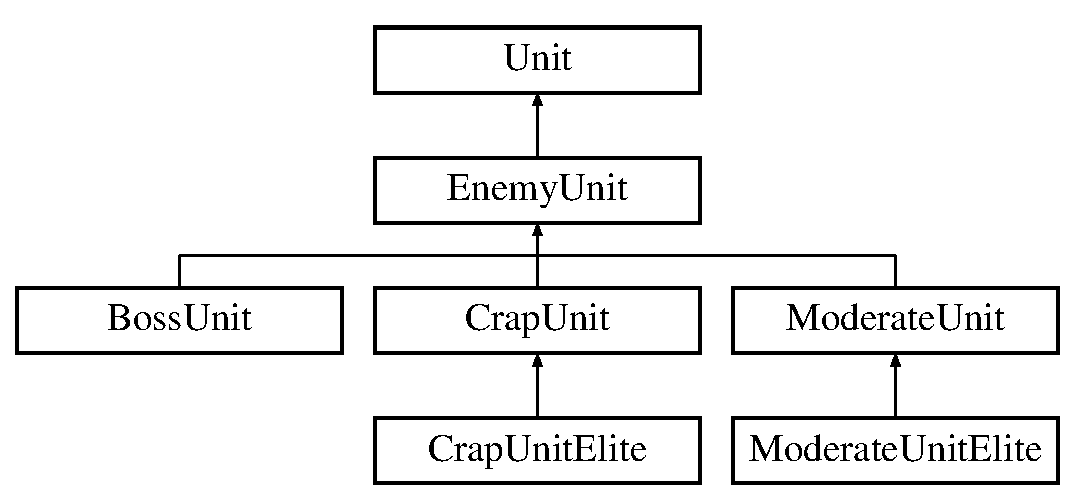
\includegraphics[height=4.000000cm]{class_unit}
\end{center}
\end{figure}
\subsection*{Public Member Functions}
\begin{DoxyCompactItemize}
\item 
\hypertarget{class_unit_ade8d5e579e440d8a24fcc06bdf876d0e}{}virtual int {\bfseries get\+Hate} ()=0\label{class_unit_ade8d5e579e440d8a24fcc06bdf876d0e}

\end{DoxyCompactItemize}


The documentation for this class was generated from the following file\+:\begin{DoxyCompactItemize}
\item 
Unit.\+h\end{DoxyCompactItemize}

\hypertarget{class_weapon}{}\section{Weapon Class Reference}
\label{class_weapon}\index{Weapon@{Weapon}}
\subsection*{Public Member Functions}
\begin{DoxyCompactItemize}
\item 
\hypertarget{class_weapon_a58073efa57ceb895524ff6d6ac9e7cd2}{}{\bfseries Weapon} (int)\label{class_weapon_a58073efa57ceb895524ff6d6ac9e7cd2}

\item 
\hypertarget{class_weapon_a82b5ccae66471ec73724ec851605b053}{}{\bfseries Weapon} (string, string, string)\label{class_weapon_a82b5ccae66471ec73724ec851605b053}

\item 
\hypertarget{class_weapon_a0b27bfcefcb412059583fef6cae5d79b}{}void {\bfseries set\+W\+Nam} (string)\label{class_weapon_a0b27bfcefcb412059583fef6cae5d79b}

\item 
\hypertarget{class_weapon_afc4aff58ba56a4d02271e8c24865cd55}{}void {\bfseries set\+W\+Bon} (string)\label{class_weapon_afc4aff58ba56a4d02271e8c24865cd55}

\item 
\hypertarget{class_weapon_aa4e777da51fb31117d9dd9671ccab9a1}{}void {\bfseries set\+W\+Typ} (string)\label{class_weapon_aa4e777da51fb31117d9dd9671ccab9a1}

\item 
\hypertarget{class_weapon_aadca77a1073527cf5d9455d6a154130d}{}string {\bfseries get\+W\+Nam} ()\label{class_weapon_aadca77a1073527cf5d9455d6a154130d}

\item 
\hypertarget{class_weapon_a0544d20db5d22fd2c83f4b716438c281}{}string {\bfseries get\+W\+Bon} ()\label{class_weapon_a0544d20db5d22fd2c83f4b716438c281}

\item 
\hypertarget{class_weapon_a64b107855e5dc16142927ad92e72ab1f}{}string {\bfseries get\+W\+Typ} ()\label{class_weapon_a64b107855e5dc16142927ad92e72ab1f}

\end{DoxyCompactItemize}


The documentation for this class was generated from the following files\+:\begin{DoxyCompactItemize}
\item 
Weapon.\+h\item 
Weapon.\+cpp\end{DoxyCompactItemize}

%--- End generated contents ---

% Index
\backmatter
\newpage
\phantomsection
\clearemptydoublepage
\addcontentsline{toc}{chapter}{Index}
\printindex

\end{document}
